
\def\layersep{1cm}

\begin{center}
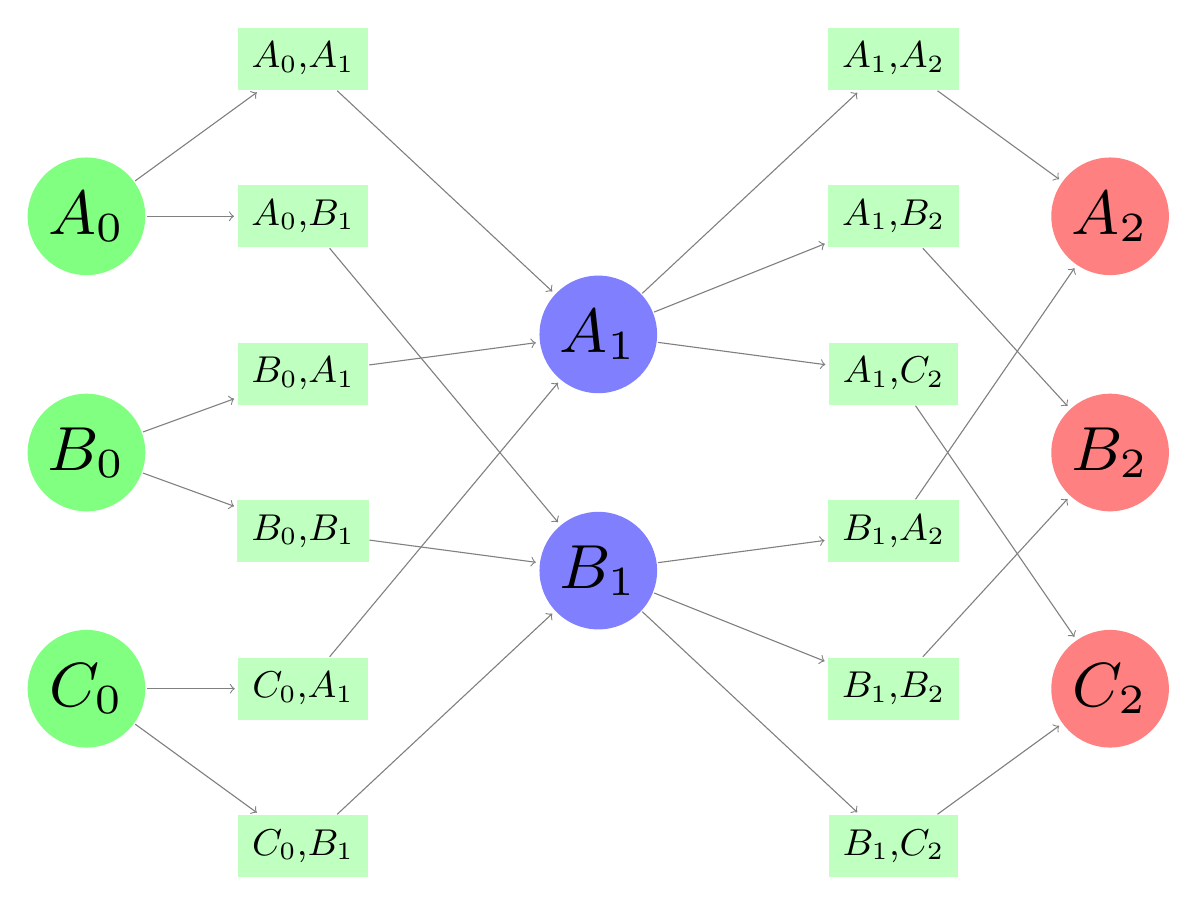
\begin{tikzpicture}[shorten >=1pt,->,draw=black!50, node distance=\layersep]
    \tikzstyle{every pin edge}=[<-,shorten <=1pt]
    \tikzstyle{neuron}=[circle,fill=black!25,minimum size=17pt,inner sep=0pt]
    \tikzstyle{input neuron}=[neuron, fill=green!50];
    \tikzstyle{output neuron}=[neuron, fill=red!50];
    \tikzstyle{hidden neuron}=[neuron, fill=blue!50];
    \tikzstyle{slave}=[rectangle,fill=green!25,minimum width = 1.5em, minimum height = 1.5em]
    \tikzstyle{annot} = [text width=3em, text centered]

    % Draw the input layer nodes
    %\foreach \name / \y in {1,...,3}
    %    \node[input neuron,scale=3] (I-\name) at (-5cm,-3*\y cm) {};

    \node[input neuron,scale=2.5] (I-1) at (-6cm,-2cm) {\small $A_0$};
    \node[input neuron,scale=2.5] (I-2) at (-6cm,-5cm) {\small $B_0$};
    \node[input neuron,scale=2.5] (I-3) at (-6cm,-8cm) {\small $C_0$};

    \node[slave,scale=1.5] (S-1) at (-3.25cm, 0cm)   {\small $A_0$,\small $A_1$};
    \node[slave,scale=1.5] (S-2) at (-3.25cm, -2cm)  {\small $A_0$,\small $B_1$};
    \node[slave,scale=1.5] (S-3) at (-3.25cm, -4cm)  {\small $B_0$,\small $A_1$};
    \node[slave,scale=1.5] (S-4) at (-3.25cm, -6cm)  {\small $B_0$,\small $B_1$};
    \node[slave,scale=1.5] (S-5) at (-3.25cm, -8cm)  {\small $C_0$,\small $A_1$};
    \node[slave,scale=1.5] (S-6) at (-3.25cm, -10cm) {\small $C_0$,\small $B_1$};

    \node[hidden neuron,scale=2.5] (H-1) at (0.5cm,-3.5cm) {\small $A_1$};
    \node[hidden neuron,scale=2.5] (H-2) at (0.5cm,-6.5cm) {\small $B_1$};
    
    \node[slave,scale=1.5] (S2-1) at (4.25cm, 0cm)   {\small $A_1$,\small $A_2$};
    \node[slave,scale=1.5] (S2-2) at (4.25cm, -2cm)  {\small $A_1$,\small $B_2$};
    \node[slave,scale=1.5] (S2-3) at (4.25cm, -4cm)  {\small $A_1$,\small $C_2$};
    \node[slave,scale=1.5] (S2-4) at (4.25cm, -6cm)  {\small $B_1$,\small $A_2$};
    \node[slave,scale=1.5] (S2-5) at (4.25cm, -8cm)  {\small $B_1$,\small $B_2$};
    \node[slave,scale=1.5] (S2-6) at (4.25cm, -10cm) {\small $B_1$,\small $C_2$};


    \node[output neuron,scale=2.5] (O-1) at (7cm,-2cm) {\small $A_2$};
    \node[output neuron,scale=2.5] (O-2) at (7cm,-5cm) {\small $B_2$};
    \node[output neuron,scale=2.5] (O-3) at (7cm,-8cm) {\small $C_2$};


    \path (I-1) edge (S-1);
    \path (I-1) edge (S-2);
    \path (I-2) edge (S-3);
    \path (I-2) edge (S-4);
    \path (I-3) edge (S-5);
    \path (I-3) edge (S-6);

    \path (S-1) edge (H-1);
    \path (S-3) edge (H-1);
    \path (S-5) edge (H-1);
    \path (S-2) edge (H-2);
    \path (S-4) edge (H-2);
    \path (S-6) edge (H-2);

    \path (H-1) edge (S2-1);
    \path (H-1) edge (S2-2);
    \path (H-1) edge (S2-3);
    \path (H-2) edge (S2-4);
    \path (H-2) edge (S2-5);
    \path (H-2) edge (S2-6);

    \path (S2-1) edge (O-1);
    \path (S2-4) edge (O-1);
    \path (S2-2) edge (O-2);
    \path (S2-5) edge (O-2);
    \path (S2-3) edge (O-3);
    \path (S2-6) edge (O-3);


    % Annotate the layers
    %\node[annot,above of=I-1, node distance=0.8cm] {1};
   
\end{tikzpicture}
\end{center}
